%Az összefoglaló fejezet
\chapter*{Adathordozó használati útmutató}
\addcontentsline{toc}{chapter}{Adathordozó használati útmutató}

A szakdolgozathoz 1 darab DVD-t mellékeltem. A lemez 3-as szintű 31 karakter hosszú fájlneveket engedélyező ISO9660 formátumú, Rock Ridge, UDF, és Joliet bejegyzéseket is tartalmaz. A lemezt kötelezően UDF-érzékeny módon kell felcsatolni, mert 2GB-nál nagyobb fájlt tartalmaz. A modern operációs rendszerek ezt automatikusan érzékelik, és ennek megfelelően csatolják fel a lemezt. A lemez gyökerében három bejegyzés található, ezeket a következő fejezetekben részletezem.

\section{Software}
Ebben a mappában különböző - a lemezen található fájlok megnyitásához szükséges - programok telepítőfájljai találhatóak. A lemez az alábbi szoftvereket tartalmazza.
\begin{itemize}
	\item \textbf{VirtualBox:} Nyílt virtualizációs szoftver, egy hypervisor. Az OVA fájl beimportálásához, és az importált virtuális gép elindításához használhatjuk.
	\item: \textbf{7-Zip:} Magas tömörítési rátával rendelkező nyílt archívumkezelő szoftver. A TAR fájl kicsomagolására használhatjuk Windows rendszeren.
\end{itemize}

\section{Szakdolgozat.tar}
Sajnálatos módon a sok kiterjesztés ellenére az ISO formátum korlátai túlságosan kötöttek, például könyvtárakra mutató linkeket képtelen kezelni, így a szakdolgozatom anyagát TAR formátumba csomagoltam.

\subsection{A TAR archívum kicsomagolása}
A TAR archívumot használat előtt ki kell csomagolni egy olyan helyre, ahova a felhasználónak van írási jogosultsága, illetve a célmappa fájlrendszere támogatja a linkeket.

\subsubsection{Unix rendszereken:}
Használhatunk bármilyen grafikus csomagoló programot, vagy a legtöbb Unix-szerű rendszerre előre telepített tar parancsot.\\
tar -xf /DVD/csatolási/pont/Szakdolgozat.tar -C /cél/könyvtár

\subsubsection{Windows rendszeren}
Sajnos a Windows nem rendelkezik olyan előtelepített szoftverrel, ami képes lenne ennek a formátumnak a kezelésére, ezért a lemezen mellékeltem a 7-Zip nevű csomagoló szoftver (Software mappán belül 32 bit: 7z1604.exe; 64bit: 7z1604-x64.exe) telepítőjét, melynek a segítségével (telepítés után) ki tudjuk csomagolni a TAR archívumot.

\begin{remark}
	A TAR archívum linkeket tartalmaz, Windows rendszeren azonban előfordulhat, hogy a felhasználóként futtatott szoftver nem rendelkezik megfelelő jogosultsággal a linkek létrehozásához, ezért indítsuk a 7-Zip archívumkezelőt rendszergazdai jogosultsággal.
\end{remark}

\subsubsection{A TAR tartalma}
Kicsomagolás után a következő mappastruktúra fogad minket:
\begin{itemize}
	\item \textbf{szakdolgozat:} Ez a mappa tartalmazza a szakdolgozathoz tartozó projektmappákat. A benne lévő Gameplayer a programhoz, míg a szakdolgozat/szakdolgozat mappa jelen dokumentum TEX projektmappája. Ez a mappa egyben egy GIT repository is, egy tetszőleges GIT klienssel megnyitva megtekinthető az összes korábbi változata ezeknek a projekteknek.
	\item \textbf{GamePlayer.jar:} Szimbolikus link a programhoz. Ezt a fájlt a Java 8 SE futtatókörnyezethez társítsuk, megnyitásával elindul a program.
	\item \textbf{szakd\_pozsgay.pdf:} Szimbolikus link, ehhez a dokumentumhoz tartozó projekt mappában lévő készre renderelt PDF dokumentumra hivatkozik. Ennek a fájlnak a megnyitása jelen dokumentum megjelenítését eredményezi.
\end{itemize}

\section{Szakdolgozat.ova}
A lemez összeállításakor kulcsfontosságúnak éreztem, hogy mind a dokumentum, mind pedig a program könnyen reprodukálható legyen. Éppen ezért létrehoztam egy Virtuális gépet, amelybe feltelepítettem minden olyan szoftvert, és komponenst, ami ahhoz szükséges, hogy a jelen dokumentumot szerkeszteni, a programot fejleszteni lehessen.\ujsor

Az OVA egy nyílt formátum virtuális gépek tárolására, a VirtualBox virtualizációs szoftver kiválóan kezeli ezt a formátumot, segítségével beimportálható, és elindítható a virtuális gép. A program telepítője megtalálható a Software/VirtualBox mappában\ujsor

A virtuális gép rendszerigénye legalább 2GB memória, és 64 bites x86-64 architektúrájú processzor. Amennyiben a virtuális gépet sikerült elindítanunk, az alább látható kép fogad minket:

\begin{figure}[ht]
	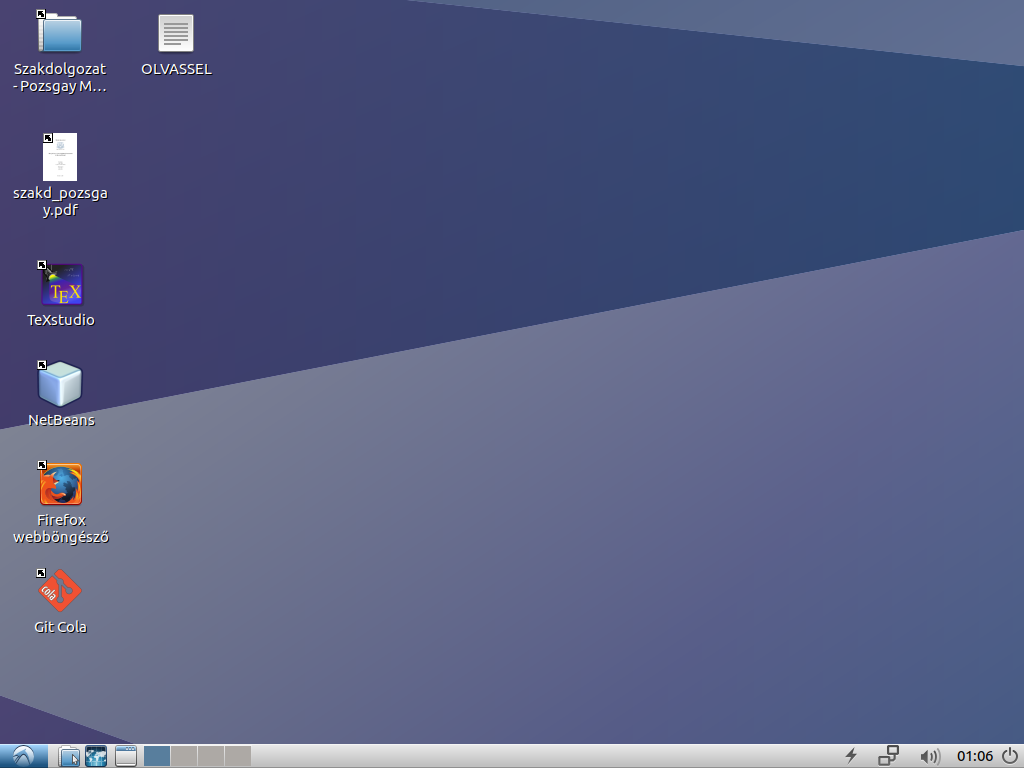
\includegraphics[width=15cm, height=11cm]{vm}
	\centering
	\caption{A virtuális gép indulás utáni állapota}
	\label{fig:vm}
\end{figure}

Az asztalon található indítóikonok mind elő vannak készítve, és a releváns projektet be is töltik induláskor, továbbá a Firefox böngészőben a könyvjelzők közé felvettem az irodalomjegyzékben található linkeket is.
